%! suppress = UnresolvedReference


\chapter{\app 的开发}\label{ch:dev}


\section{项目的开发环境与开发工具}\label{sec:env}

本项目包含了多种语言的代码的编写,不同语言所使用的开发环境与工具有重叠部分也有不同部分,并且在本地环境与持续集成环境中的配置也有一定差异。

\subsection{通用的环境与工具}\label{subsec:common-env}

项目中的所有代码都使用了Git进行版本控制,项目的源代码托管在GitHub上,并且使用了GitHub Actions作为持续集成工具,开发过程中也遵循了GitHub推荐并支持的pull request、release等工作流程。Git的提交信息遵循约定式提交(Conventional Commits)规范,版本号则按照语义化版本(Semantic Versioning)规范进行管理。新版本的发布及版本号的更新基于Google的Release Please工具半自动地进行,该工具同时用于更新日志的自动生成。为了方便使用GitHub,在本地安装并使用了GitHub CLI与GitHub Desktop。

项目的各部分代码均使用Codecov进行测试覆盖率的统计追踪,使用Renovate进行依赖项的自动更新,使用Restyled自动格式化代码,使用CodeFactor进行代码质量的检查,并使用Sentry来自动收集并上报错误信息。另外,各部分代码的编写都借助了GitHub Copilot来提供更智能的代码补全。

\subsection{Dart及Flutter的环境与工具}\label{subsec:dart-env}

项目开发基于最新的稳定版的Flutter SDK,在开发过程中其版本进行过几次更新,截止本文撰写时使用的是Flutter 3.7.10。Dart SDK使用的是捆绑于Flutter SDK中的对应版本,并未单独配置。

开发过程中,在本地使用了IntelliJ IDEA作为Flutter开发的IDE,安装了Flutter插件与Dart插件来提供相应的支持,并额外安装了Flutter Freezed Snippets、Flutter Intl等插件来提供更多相关功能。为了获得对移动平台开发的支持,在一台Windows设备和一台macOS设备上分别额外安装了Android Studio和Xcode及其对应移动平台设备的模拟器。

在持续集成环境中,基于subosito开发的flutter-action配置了Android和iOS平台的应用安装包的自动构建发布。除Flutter SDK自带的静态分析、代码测试等工具外,额外使用了社区开发的Dependency Validator包来检查依赖项是否有缺少或冗余。

\subsection{\LaTeX 的环境与工具}\label{subsec:latex-env}

在本地安装了\TeX\ Live 2023,并使用安装了\TeX iFy插件的IntelliJ IDEA作为IDE。在持续集成环境中,使用了xu-cheng提供的最新版\TeX\ Live的Docker镜像进行文档的编译,并配置了相应的自动发布。

\subsection{C++的环境与工具}\label{subsec:cpp-env}

项目中对于Pan-Tompkins算法和基于LibTorch的算法的开发使用了不同的环境。由于开发时主要使用的是Windows系统,所以在Pan-Tompkins算法的开发过程中使用了MSVC工具链。而基于LibTorch的算法则因为Windows平台的LibTorch分发版区分了调试与发布版本而较难使用,所以使用了安装在WSL2中的GCC工具链。两者都使用CLion作为IDE,一个直接安装在Windows系统中,另一个安装在WSL2中然后通过JetBrains Gateway连接。

在持续集成环境中,使用aminya提供的setup-cpp工具来安装必要的依赖。两个仓库中的代码均在最新的Ubuntu环境下使用GCC与CMake工具链进行编译,然后基于Gcovr进行代码覆盖率的统计。

\subsection{Python的环境与工具}\label{subsec:python-env}

对于Python环境的管理使用了Mamba,Conda的一个更优秀的替代工具。在本地安装了Mambaforge用于依赖管理,持续集成环境中则使用provision-with-micromamba工具。Python代码的测试与覆盖率生成基于pytest和pytest-cov工具。本地开发的IDE选择了PyCharm。


\section{Pan-Tompkins算法的实现}\label{sec:pan-tompkins}

本应用为用户提供了实时的心率显示。因为所使用的基于LibTorch的算法无法实时给出心电分割结果,所以有必要另外使用一种实时在线算法来进行心率的统计。

Pan-Tompkins算法\cite{panRealTimeQRSDetection1985}可以用于检测心电图中的QRS波群。一次正常的窦性心律的组成如图~\ref{fig:sinus-rhythm} 所示,其中的QRS波群位于心电图中最明显的尖峰处。此功能使得Pan-Tompkins算法非常适合用作心率测量。

\begin{figure}[ht]
    \centering
    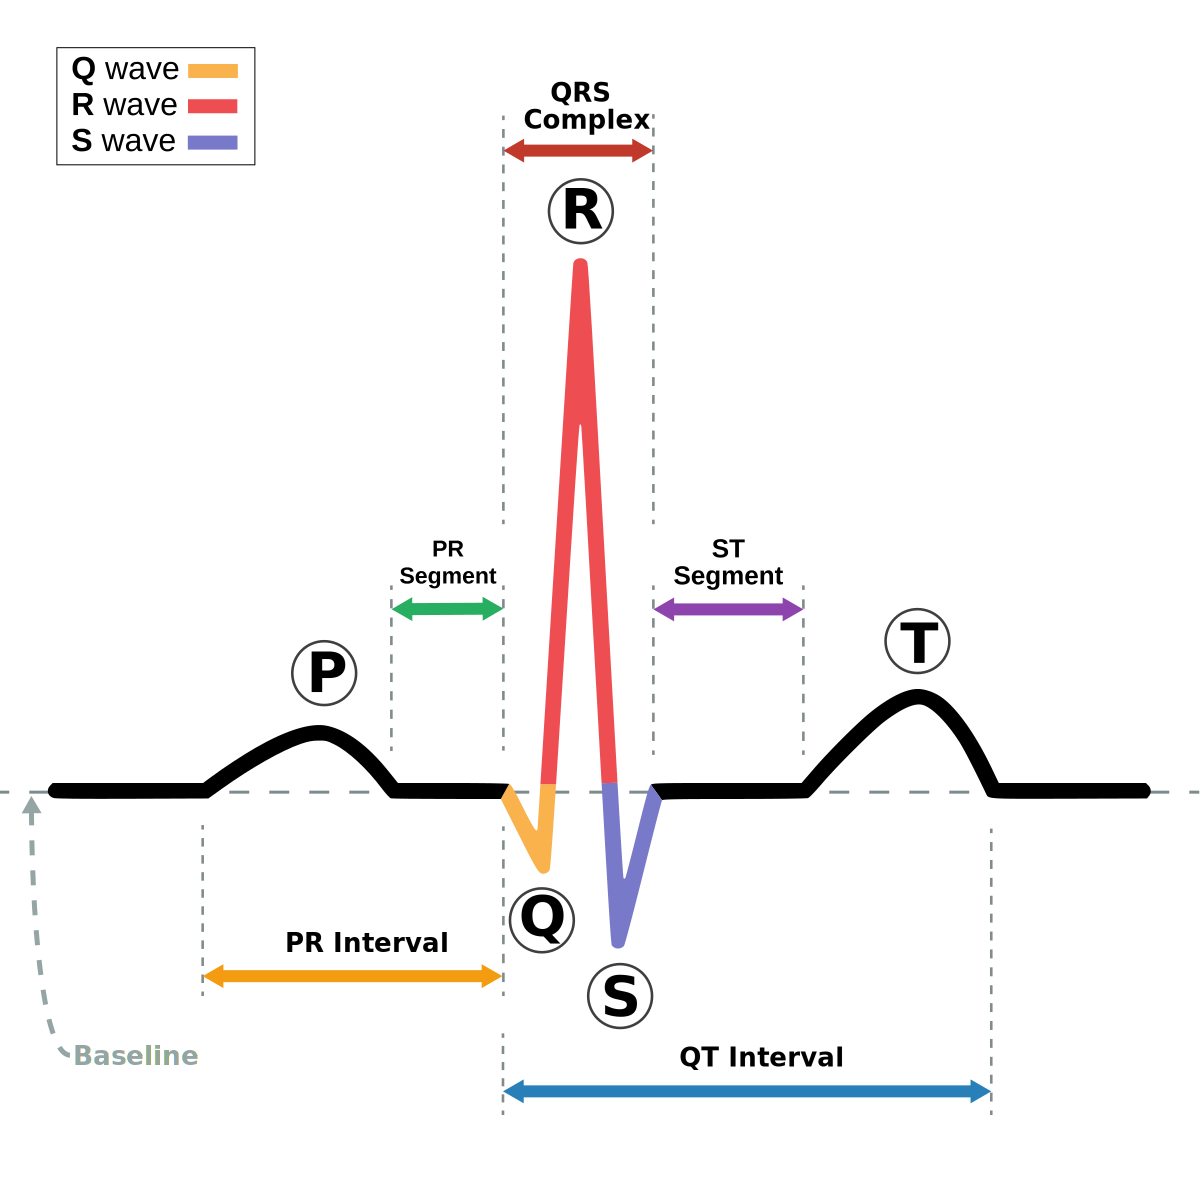
\includegraphics[width=.75\textwidth]{../assets/SinusRhythmLabels}
    \bicaption{正常窦性心律的心电图}{ECG of a heart in normal sinus rhythm}
    \label{fig:sinus-rhythm}
\end{figure}

该算法是心电分析中最经典的算法之一。于1985年被提出后,有许多人对其进行了各种各样的改进。由于算法的原始版本已经有很高的准确率(原作者给出的统计结果为99.3\%),同时本应用仅将其用作心率检测,没有很高的准确率要求,所以出于实现较为简单的优势而直接使用了原始版本的算法,而非其他人的改版。

由于Pan-Tompkins算法的应用非常广泛,多年以来,已经有大量开发者用各种语言各种方式对其进行了实现。为了不进行无意义的额外工作,本项目在Pan-Tompkins算法的实现过程中并非从零开始编写,而是基于已有的实现进行了修改。经过检索对比,发现rafaelmmoreira为该算法编写的C语言实现\footnote{\url{https://github.com/rafaelmmoreira/PanTompkinsQRS}}的代码质量较高,以MIT协议开源,并提供了充分的注释文档以方便理解,因此本项目以该版本实现为基础按项目需要进行了一些修改。

首先,将该实现由C语言迁移至了C++。除了将在C++中无法通过编译的特性(比如动态数组大小)进行了修改外,还将一些内容的写法改为了C++中惯用的写法,包括将使用宏定义的常量改为 |constexpr|、将 |fopen| 相关的写法替换为 |std::ifstream| 等。

之后,对该实现的输入输出方式进行了修改。在原始版本的算法中,程序开始运行时会打开两个文件作为输入输出。为了方便Dart调用,需要将输入输出方式改为直接通过参数和返回值进行。原作者已经考虑到需要修改输入输出方式的需求,并从算法中提取出了 |dataType input()| 和 |void output(int out)| 两个函数。原始情况下,算法会在需要读入新数据时调用 |input|,在分析结果就绪后调用 |output|,两者之间并不同步,而是使用了异步回调。跨语言实现异步回调虽然并非完全不可行,但相比简单的调用后直接返回的流程更为繁琐,且没有太大收益。经过分析,发现该算法实现的主体部分是一个无限循环,在循环的开头会调用 |input| 获取采样点数据,在循环中间的多处会调用 |output| 后进入到下一次循环。为了将其改为单次调用后直接返回的方式,将该循环的内容提取为了另一个函数,并将需要在循环之间保留的状态由函数内的局部变量暂时改为了全局变量。同时,将输入与输出进行同步,以略微降低算法精度为代价获得了更及时的检测结果。

在该实现的原始版本中,采样率是以常量的形式硬编码在算法之中的。但是,实际调用该算法进行分析时,可能会以不同采样率的数据进行输入。一种可能的方式是将算法复制多份修改常量后分别编译,但比较繁琐。另一种方式是将该常量改为算法的参数,从外部传入。由于算法中有很多常量和变量的值与采样率有关,因此为了方便将其作为参数,将上一个步骤中提取出的全局变量与函数封装成为了类,并将采样率作为该类的构造函数的参数。这一改动也解释了之前为什么选择将C语言的实现迁移至C++而非直接使用C语言进行重构,这样可以利用C++的强大特性来简化代码的编写难度。

在最终版本的算法中,对外提供了两个函数作为接口,分别是 |void init(int fs)| 和 |bool panTompkins(float sample)|。包含相关状态与方法的类被简单地命名为 |PanTompkins|。程序中维护了一个 |std::optional<PanTompkins>| 类型的全局变量,用于存储算法的状态。在调用 |init| 时,如果全局变量目前为空或者存储的算法的采样率与传入的参数不同,则会创建一个新的算法实例并存储在全局变量中;如果全局变量目前不为空且存储的算法的采样率与传入的参数相同,则不会创建新的算法实例,而是直接复用旧的实例,以减少不必要的开销。由于用户通常不会频繁更换使用不同采样率的设备,此优化的效果是比较明显的。在调用 |panTompkins| 时,会断言当前全局变量不为空,也就是要求调用者必须先调用过 |init| 再调用此方法;之后,会将传入的采样点数据转发至算法实例的对应方法,该方法会返回一个布尔值,表示是否检测到了新的QRS波群。

在算法的测试过程中,发现其偶尔会对于同一个心拍输出两次或更多相近甚至相邻的 |true|,导致计算出的心率可能会突然提升至每分钟上千次。由于难以确定是在算法的哪一处出现了问题,所以在算法之外对于其输出结果设计了两层额外修正,而没有修改算法内部的执行逻辑。第一层修正是为算法输出的QRS波群设置最小间隔,该间隔的计算方式如下:

\[
    leastSamplesBetweenQrs = \frac{60}{maxHeartRate} \times fs
\]

其中,\(leastSamplesBetweenQrs\) 表示连续两个QRS波群之间至少需要间隔的采样点数。当算法返回了 |true| 时,会将当前的采样点与上一次检测到QRS波群的采样点进行比较,如果两者之间的采样点数目小于 \(leastSamplesBetweenQrs\),则会忽略该检测结果,否则会将当前的采样点作为最后一次检测到QRS波群的采样点。60表示一分钟的秒数,\(maxHeartRate\) 表示最大心率(单位bpm),\(fs\) 表示采样率(单位Hz)。关于人类的心率上限,最流行的说法是220减去年龄。考虑到患者应该不会在心率超出此上限的情况下还有使用本应用观察自己心率的需求,同时为了不需要获取患者的实际年龄就可以运行算法,在实现中将\(maxHeartRate\) 设置为了常量220。经过测试,该修正可以有效地解决算法输出的QRS波群之间间隔过小导致心率上千的问题。

此外,在最终的心率显示部分也增加了一层修正。该层修正是在前述过滤方式未能完全排除算法的错误输出的情况下的缓冲。考虑到人类的心率的变化应该是相当平滑的,不太可能在相邻几个心拍之间产生非常大的变动,应用在最终将心率计算结果展示给用户的时候会先与之前的结果进行比较,如果相差超过10bpm,则会将显示结果改为上一次结果加上或减去10bpm(取决于心率是突然上升还是突然下降),但不改变底层数据的实际值。通过这种方式,可以有效地避免因为算法的错误输出导致心率突然上升或下降的情况,同时在心率真的在短时间内发生了较大的变化时,也能够在数次心拍后将心率恢复到正确的值。

应用对于心率的计算是根据最后两次检测到的心拍的间隔时间,所以另一个考虑过的修正方案是使用较多心拍之间间隔的平均值来计算心率。这种方案的效果与原理和上一段说明的方式类似,都是对心率变化进行平滑处理,滤去突变。相比起来,这种方案需要将过去的更多心拍纳入计算,但相比之前的方法在效果上没有明显的优势,所以在实现中没有采用。


\section{智能检测算法的移植与优化}\label{sec:ai}

Pan-Tompkins算法只能给出心拍的位置,但无法确定心拍的类型。同时,其作为在线算法,虽然有能实时输出结果的优点,但准确率相较离线算法也更低一些。由于用户对于分析报告的查看没有实时性非常高的需求,因此应用使用基于人工智能的另一种算法来对心电数据进行分析。

所用算法的原始版本使用Python实现。对于将其迁移至C++的过程,考虑过两种方案。其一是先将Python代码原样翻译成C++,再对C++代码进行重构以满足项目需求;这种方案的优点在于比较容易按C++的风格对代码进行重构,而缺点在于需要翻译的代码量比较大故容易出错,而且其中包含很多最终不需要使用的代码以及难以在C++中找到对应替代的依赖项。因此,本项目采用了与之相对的另一种方案,即先对Python代码进行重构,再将重构后的代码原样翻译成C++;这种方案可以最小化翻译代码步骤的工作量,并可以事先编写单元测试来保证重构过程不会破坏代码的正确性;其主要缺点则在于需要在重构过程中注意避免使用难以在C++中实现的特性,比如对同一变量进行多次不同类型的赋值\footnote{严格来说,这可以通过std::variant或union等方式实现,但会失去一部分静态类型检查的好处。}等。

首先执行的步骤是对代码的格式进行统一。在原始版本的代码中,命名、空格等格式均混合使用了多种风格,不便阅读。因此,首先对代码使用Black工具进行了格式化,使得代码的空格、换行等风格更加统一。然后利用PyCharm的重构功能对代码中变量、函数等的命名进行了修改,使其遵守Python官方的PEP-8规范中对命名的相关要求。此外,在该步骤中也移除了PyCharm能够直接检测出的一些未被使用的导入项;自动优化导入后发现代码无法继续正常运行,排查发现代码中使用类似反射的方式使用了部分导入的内容,因此未被PyCharm检测到;为该类实际上被使用的导入项添加了注释,以抑制PyCharm的误报。

之后进行的是对算法的输入输出方式的优化。在原始版本中,算法的每个步骤都是从磁盘文件读取数据作为输入,之后把其结果写入另一个磁盘文件。这种方式虽然编写简单,但会导致数据在各个步骤之间的流向非常不清晰,并且在性能上有所损耗。最关键的是,这种输入输出方式使得难以为各个步骤编写单元测试。因此,优先调整了代码中数据的传递方式,使之仅在主函数中从磁盘文件读入,之后各个步骤均通过参数与返回值直接传递,最后再在主函数中将最终结果写入磁盘文件。这样以来,就可以通过替代主函数来为算法编写单元测试,方便后续重构。该步骤完成之后,对比了最终的磁盘文件与原始版本的输出,发现了一些不一致,经研究讨论后发现是出于原始版本的一些bug,修复后可以得到一致的输出。据此可以判定该步骤并未破坏算法的正确性(反而修正了原本存在的缺陷),而此后的步骤都可以通过持续集成中自动运行的单元测试而非手动对比来保证这一点。

原始项目中包含非常多的代码文件,但是经过覆盖率检测,发现在算法执行的过程中大部分代码都没有被执行到。经过仔细测试、分析,发现有许多代码是多余的。于是删去了无意义的代码,这包括原项目中的数个目录、一些文件、以及某些文件中的部分代码行。之后,发现有部分模型等资源文件也未被读取过,将这些文件也进行了清理。完成对于未使用文件的清理后,对项目中各个文件的位置进行了调整,将代码文件与资源文件等分别移至单独的目录中,方便后续继续重构。

该算法原本使用了一段长达24小时的动态心电数据进行测试,这可以较为充分地测试算法对于各种类型的心电数据的表现,但也导致测试时间很长,单次执行需要数分钟,在性能较差的持续集成环境下甚至需要更久。由于代码每次进行更改时都要重新运行测试以保证正确性,为了减少在测试步骤的等待时间,提高开发效率,将数据截取了前10分钟来进行更快速的测试。

下一个步骤是进行更细粒度的重构。由于原项目代码的组织结构较为混乱,为了方便后续处理,首先将所有代码文件合并至单个文件之中,去除了多个代码文件之间的导入。在合并的过程中以及合并完成后,发现各个文件中存在部分逻辑相似甚至完全相同的代码,对这些重复的代码进行了合并,提取了共用的方法。并且,对一些未使用的参数进行了删除;对在所有调用中均传递了相同值的参数(比如重采样的目标采样率被固定为250Hz)进行了简化,仅作为全局常量,而不在层层调用中进行传递。在该步骤中,也对方法中一些不符合正常编码习惯的写法进行了替换,比如将 |flag == False| 改为 |not flag|(C++中为 |!flag|)、手动打印错误消息改为抛出异常等。此外,对一些与最终结果无关的调试代码,比如基于 |tqdm| 打印算法执行进度的代码,进行了删除,并消去了相关依赖项。最后,将简化完毕的代码重新按执行步骤分割为多个模块,分别存储于单独的代码文件供主函数调用,并将仅在某一步骤使用的函数设为模块级别的私有函数,以提高代码的内聚性。

将代码迁移至C++前的最后一个重构步骤是为参数、变量、返回值等添加类型标注。虽然Python是动态类型语言,但通过类型标注,仍然可以获得静态类型检查的优势。在该步骤中,使用Mypy工具进行了严格的检查,固定了每个变量、参数的类型,对同变量多次赋值为不同类型的情况进行了变量拆分。在这一步骤中也借助类型检查发现了原始代码中的一处笔误,该笔误所处代码所代表的情况刚好在测试数据的执行过程中未出现过,所以之前未被发现。之后,对错误进行了修正。

得益于上述的重构,以及LibTorch、NumCpp等库的接口设计的友好性,迁移过程的工作基本都在于翻译语言功能,很少涉及代码逻辑的修改。然而,在将代码原样翻译成C++后,发现在原本在Python中可以正常使用 |torch.load| 加载的模型文件无法在C++中使用 |torch::load| 读取。检索并查阅相关资料后,发现需要先将模型转换为TorchScript格式以消除Python依赖。在转换过程中,为了适应TorchScript的限制,对模型代码进行了微小重构,如将 |for| 循环进行展开等。

在迁移过程中编写的LibTorch相关代码是在Linux环境下进行调试的,这是考虑到在移动端调试C++代码较为不便,并且C++代码具有跨平台性,在Linux下能够正常运行应该就意味着可以在其他平台也正常运行。不过,在将于Linux平台下调试完成的代码移植至移动平台时还是遇到了麻烦,其原因在于C++的跨平台性仅在源代码级别成立,而编译后的二进制文件并不能跨平台使用。而在该部分算法的各种依赖项中,LibTorch的分发方式与其他依赖不同,虽然官方也提供了开源代码,但主要的安装方式是下载并解压预先编译好的静态链接库以及相关的头文件等。但是在官网的下载页面\footnote{\url{https://pytorch.org/get-started/locally/}}中,只提供了三个桌面端系统的LibTorch下载,而没有提供移动端的LibTorch。

为了获得能在移动端使用的LibTorch,考虑过两个方案,一是从源代码自行编译,二是寻找已经编译好的版本。由于LibTorch项目规模庞大,自行编译的方式繁琐且耗时,所以优先考虑了使用已经被编译好的版本。在经过了一些寻找与尝试后,发现PyTorch官方提供的PyTorch Mobile中存在LibTorch的相关文件;事后想来这是很自然的,因为PyTorch的各种版本都是为其底层的C++实现提供其他语言的接口,那么LibTorch作为C++版本的接口也很可能会在其中使用到。在移动端的构建过程中,首先将PyTorch Mobile作为依赖项正常下载,然后并不直接使用,而是将其解压并将其中的LibTorch头文件和链接库复制至构建目录中,在C++的编译过程中对相关的头文件目录进行包含并将其链接库与算法代码进行链接。

\section{实时心电模块的实现}\label{sec:real-time}

\todo{实时心电模块的实现}


\section{历史心电模块的实现}\label{sec:history}

\todo{历史心电模块的实现}


\section{分析报告模块的实现}\label{sec:analytics}

\todo{分析报告模块的实现}


\section{设备管理模块的实现}\label{sec:device}

\todo{设备管理模块的实现}


\section{应用设置模块的实现}\label{sec:settings}

\todo{应用设置模块的实现}


\section{其他功能的实现}\label{sec:other}

\subsection{路由功能的实现}\label{subsec:router}

\todo{路由功能的实现}

\subsection{本地化功能的实现}\label{subsec:l10n}

\todo{本地化功能的实现}

\subsection{开发者工具的实现}\label{subsec:dev-tools}

\todo{开发者工具的实现}

\subsection{应用信息显示功能的实现}\label{subsec:about}

\todo{应用信息显示功能的实现}
